ABSTRACT

%****************************************
% SAMPLE ABSTRACTS

% Bu çalışmada, ne kadar itici bir kavram olsa da, çöplük olgusunun çirkinlikten güzelliğe ulaşarak estetik bir haz uyandırması amaç edinilmiştir. Iticici gözüken bir konunun resim diliyle anlatımı ile tersine çekici ilginç bir sanat konusu olabileceğinin somutlaştırılması amaçlanmıştır. Sanatçı bir anlamda doğada yaşamda bulunan küçük ayrıntıları, sanatsal bir gözle yaklaşarak gösterebilendir. Resim için konu denince hep bildik tanıdık nesneler, belli bir düzenleme anlayışı (Natürmort) ya da idealize edilmiş konular, temalar akla gelir. Oysa önemsiz gibi gözüken itici karmaşık konular bile sanatsal kaygılarla ele ahnabilmelidir. Önemli olan, bu konalara estetik yaklaşım ve izlenen anlatım yol ve teknikleridir. Özgün baskı dallarından kazı resim (gravür) tekniğinin ele alınan konunun görselleştirilmesinde, anlatımında en uygun teknik olmasıdır. Çünkü her sanatçı kendi doğasına en uygun olan teknik ve malzemelerin olanaklarıyla kendini en rahat biçimde ifade etme olanağı bulur. Kendine özgü bir biçim ve anlatım diliyle dile getirmek gerçekleştirmek çabalan özgünlüğü yakalamak içindir. Bu çalışmada özgünlüğü yakalamak, çöplük olgusunun oluşturduğu dinamik yapı, objelerin biçimlerine bağlı kalmadan plastik dille görselleştirilmiştir. Seçilen teknik doğası gereği raslantısal tadlarada olanak vermektedir. Oluşturulan resimlerde durağan bir dengeden çok dinamik biçim ilişkilerine dayanan gerilimli bir etkinin yakalanması amaçlanmıştır.

% ON THE RELATIONSHIP BETWEEN IMAGES AND WORDS AND THEIR RELATION TO BODY AND PERCEPTION
% Prehistoric man created a mark and throughout the history this mark evolved and bifurcated into two: a word and an image. While images were cherished, words were set apart from images. 
% This thesis attempts to look at the relationship between images and words through seeking their connection to perception and body. It investigates how image-word dichotomy occurred and how this dichotomy obscured the connection between writing and body. The thesis also examines different approaches to overcome this phenomenon in the context of Modern Art. 
% By examining my artwork within this framework, it argues that it is possible to embody the inseparable relationship between images and words through reconnecting with the body’s primordial existence.

% ALTERNATIVE PHOTOGRAPHY IN THE DIGITAL AGE: PERFECT PHOTOGRAPHS IN AN IMPERFECT WAY
% This thesis explores the possibility of an alternative future of photography from the union of digital and chemical domains of the photographic medium. The historical photographic processes known as Cyanotype, Salt print and Vandyke Brown are employed for this project in conjunction with the modern inkjet printer produced digital negatives. 
% As being highly sensitive to the variables during the process, each alternative photographic print exhibits a visual uniqueness. In this aspect, there is conceptual correlation with the visual uniqueness of alternative photographic processes and the visual uniqueness of albinism. Emphasizing the human element in subject, vision and craft of making photographs, this project aims to produce unique photographs of a visually unique subject.

% LAND ART ON THE BORDER BETWEEN TOPOLOGY AND ATOPOLOGY
% The purpose of this study is to discuss the Land Art movement from a topological and atopological perspective. In order to establish an extensive understanding of the matters of topology and atopology, Arkady Plotnitsky’s formalization of quasi- mathematical thinking, which is derived from Jacques Derrida’s philosophy, is treated in detail. The artistic stance, Robert Smithson, as a major figure of Land Art movement is analyzed both from the artistic and the theoretical perspectives. Thereafter, an algebraic reading of the Smithsonian conceptualization is executed in order to illuminate the liaison between the Land Art movement and the matters of topology and atopology. Finally, the thesis project, Nonlocalizable Displaced Mirrors depicts the whole attitude, which is taken throughout the study, towards the issue of Land Art on the Border between Topology and Atopology.

%........................................


INTRODUCTION

% Bence introductionda çöpün farklı şekillerde ele alınabileceğini bir şekilde göstermek gerekli. Burdaki genel geçer yaklaşımdan bahsetmek gerekli.
% Ele aldığımız çöp insanların çöpleri, günlük kullanımdaki çöpler. Çok da değerli olmayan yerine yenisi koyabileceğimiz çöpler. 

% Western societies from periods where manual labor and long struggle required in production process and materials are reused and transformed again and again, have reached to periods where production process speeds up and becomes more accessible. Consumption habits have changed radically and have created piles of trash that is not obvious how to reuse them. In this work the practice and process of reusing and transforming trash which is an alternative to today's existing production and consumption habits is investigated. Stages and expression of this practice is examined with my artwork in the context of art.

% Konunun dikkat çekici ilginç kısımları. Interesting points of the topic. Facts about the trash. Changes through the time.
% Konu hakkındaki temel bilgiler.
% Konunun ele alınan kısmı.

% Çöp ve dönüşümden bahsetmek gerekli. Çöp nedir? Dönüşüm nedir? Çöpün bir dönüşümü var mıdır? Var ise bu nasıl bir şeydir? 
% Introduce as an discussion. Trash is valueless? really? is it just a sculpture? Tons of different approaches to the trash. 

% Bu trash in every sıralamasını neden yapıyorum? Genel bir çerçeve çizmekten çok aslında evrensel bir konu olduğuna değinmiş oluyorum. Peki bu çok açık bir şey mi? Yani aslında çok da açık olmayan bilgilerek vererek yaparsam olmayabilir. Evrensel olmasının benim için ne önemi var. Yaşamımızın bir parçası demek. Tamam da buna karşı bir şey mi var. Ben göremiyorum açıkcası. Herkes bunu biliyor. Farkında mıyız. Ama farkında olmak istemediğimiz bir şey ki sürekli kendimizden uzaklaştırıyoruz. O zaman bu gerçekleri aslında ne kadar biliyoruz. Ama bunları bilmek böyle davranmamız gerektiği anlamına mı gelmektedir? Aslında yabancı olmadığımız ama uzak durduğumuz bir konu. Belki de sırf bu yüzden kaçırdığımız bir sürü şey olabilir.

% Aga çöpe farklı yaklaşımlar var. O yüzden background information olarak burada verilebilir ve scope belirlenebilir. Tam da bu noktada ise purpose kısmına geçilebilir. Çöpe nasıl yaklaşıyorlar falan filan. İşte ben tam da bu noktada sanatta nasıl yaklaşılmıştır dicem. Hatta basitçe sanatta bu tür işlere 


%****************************************
% It is a justification of the work. 
% What is trash? Who does call it trash? 
% Is it possible to transform it? How? Which methods?
%........................................


% Çöpün sanat işlerinde kullanılmasının önemi ne? Bunun karşısındaki şey nedir? Diğer alanlardaki yaklaşımlar bir şey üretemiyor mu? Bu tezin önemi ne? Birilerinin bıraktığı boşluğu doldurmak mı? Ya da benim yaptığım işin önemi ne? 


% ben bunu konuyu bir eylem olarak mı ele alıyorum.


% Önceki işlere değinmek gerekli. Bu alanla ilgili yapılmış. Mesela ne var. İki tane tez buldum aslında tam da bu konuyla ilgili. Önceki işler olacak, yetersiz eksik yanları olacak ve ben onlara belli başlı eklemeler yapacağım.


%****************************************
% Some comments
% Burada önemli olan şey soru veya sorgulanan şey. Bu soru projeye yön verecek. Yazılı tez ise bunun doğrulamasını, üretilen işin kavramsal ve kuramsal çerçevesini belirleyecek. Tartışmalar ne üzerine olmalı bu durumda? 
% The project aims to what? and what needs to justify what it questions? 
% At this point, the question of what will be in the future of photography has to be asked. Bu çok önemli, bir şeyler hazırlayıp neyin sorgulanması gerektiğini sormak gerekli.

% Tipografi ve ideoloji arasında bir ilişki vardır. Fotoğrafın geleceği? Kelime ve imaj arasındaki ilişki, beden ve algı üzerinden incelenebilir? kelime ve imaj arasında bir problem olduğundan bahsediyor. Sanat işlerinde çöp kullanmak toplum tarafından atılan şeyi tekrar kullanılabileceğini gösterebilir. Toplum ve çöp nispeten bir problemli bir durum. Burada bir dert var. Atılan tüketilen manalar var. Sanat bunları provoke mi ediyor. Peki ya ben ne öneriyorum, yani aslında bir şey önermem mi gerekiyor? Sanat ve çöp arasında nasıl bir ilişki vardır? Çöp ile diğer nesneler arasında nasıl bir ilişki vardır? 

% Zaten hali hazırda sanatçılar bunu yapıyorlar, tez aslında bunları inceliyor olabilir ama tez aslında benim işimi inceliyor. İş neyi soruyor ise aslında tez de onu soruyor. Yapılan işlerle sorulan sorular arasında bir bağlantı var. Bu noktada aslında benim işin neyi sorguladığını bulmam gerekli. Çöp dönüştürülebilir, sanatsal bağlamda. (Çok geniş değil mi abi sanatsal bağlamda demek? Çöp de çok geniş bir konu.) Konuyu bir şeklide daraltmak gerekli. Çöp sanat işlerine girmiştir. Çöp dönüştürmek aslında bir artistic acte dönüşüyor. Tezde bunu anlatıyor. Aga bu artisctic act dediğin şey de ne oluyor. Çöp dönüştürmek ne oluyor?

% Çöpe yeni bir alternatif yaşam üretmek gerekli! Neden böyle düşünüyorsun? Çünkü sürekli çöp üretiyorsun ama bir yandan da bundan dert yanıyorsun. Zizek işte bu konuya el basıyor. 

% Aslında hepimiz bir şeyleri dönüştürüyoruz! Neden böyle düşüyorsun? Örnekleri nelerdir? Bricologe bu iddayı destekler mi? Nesnleri üretim amaçlarından farklı amaçlar için kullanmak yeni bir şey değil. (Ama zaten ben sanat amacıyla kullanılmasından bahsedeceğim.) Belki bunu belirtmek için mantıklı olabilir. Ama burada bir farklılık var olamalı. Diğerinden ayıran diyeceğim ama öyle bir fark aramamak gerekli bence. Sanat o farkı yıkmak için uğraşıp duruyor. Belki de bu uğraşa katkısı bu olabilir bu işin. Bir şeyleri dönüştürme potansiyellerimiz olduğunu düşünebiliriz. Dönüştürme dediğimiz şey aslında hangi noktada açığa çıkıyor. Bir ihtiyaç anında, kaçış anında, ya da yeni alternatifler ararken mi?

% Çöpün dönüştürülmesi ne olaki? Buna bir şekilde girişte yer vermek gerekli. Çöpün market içindeki hareketi mi? Ya da aslında çöpün yaşamı. Belki de bu olabilir. Çöpün nasıl oluştuğu vs. Fabrikada üretilmesi. İnsanlara dağıtılması. Ve sonra çöp olması. Çöp dağları oluşması. Çöp kutusunda yer alması. Neler yok ki çöp kutusunda. Bir sanatçı çöp kovasına attığı sanat işleri. Sanat işleri çöplükleri vs. Çöp kavramı aslında o kadar çok şey için geçerli ki? İşte bu çok çeşitli çöp kavramını ele almak gerekli. Yani objeler bir şekilde farklı konumlarda mekanlarda yer değiştiriyorlar. Bazen çöp oluyorlar bazen değerli vs.

% Bir bir çeşit çöp var. Bunlar binbir çeşit davranış sonucunda oluşuyorlar. Bir işlemin sonunda ortaya çıkan son ürün. Çöp konumuna gelmesi vs. Kime göre çöp neye göre çöp. Ama işte ortada bir konsensus yok. Başkaları da farklı şekilde görüyor. Birine göre çöp diğerine göre ise bir hazine.

% Dönüşmek ne oluyor peki bu durumda. Bir durumdan başka bir duruma geçmesi. Farklı bir anlam, amaç kazanması olabilir mi? Mesela pisuvar dönüşmüş müydü? Gazeteyi kolajda kullandığım zaman gazeteyi dönüştürmüş mü oluyorum? Hangisi dönüştü? Zaten buradaki açık bir şekilde açığa çıkıyor aslında. Her ikisi de dönüşmüş oluyor. Farklı bir kullanım alanı bulmak. Farklı niyetlerle kullanmak olabilir belki de. Bir şeyin ne zaman dönüştüğünü iddia edebilirsin.

% Agnes varda neyi anlatıyor: Toplayıcılık hala devam ediyor, bu toplayıcılar arasında sanatçıları da geziyor, çünkü onlar da topluyorlar. Onlar da o çöplerde farklı şeyler görüyorlar. Kendi de mesela çöpe atılmış bir şeye anlam yüklüyor. Kendisininde aslında bir toplayıcı olduğunun farkına varıyor.


%****************************************
% JUSTIFICATION (Gerekçesi)
% Eğer bir şeyin justificationından bahsediyorsak ben neleri iddia ediyorum:
% - Çöpü dönüştürdüğümü. Öncelikli olarak o gerçekten çöp mü? Sonrasında ise gerçekten dönüştü mü? (throw away culture çöpü anlatsa. rubbish theoryde dönüşümü anlatsa)
% - Peki neden bu işi yapıyorsun. Alternatifi aramak. Değer bulmak, değer bulunabilceğine inanmam aslında. Belki de değer üretmek için o değerleri yıkmak gerekli. Çöpe atıldığında bu yüzden bazı değerler yıkılıyordur. Artık yeni değerler vermek için gerekli yapı oluşuyordur o zaman. O yüzden çöpe atılması önemli. Bir yerin sonuna gelmiş olması aslında belki de yeni bir başlangıç olması için önemli olabilir. Çöplüğün bir başlangıç olması. Batırdığımız bitridiğimiz yerden yeni bir başlangıç. Çöpü üreten üretilmiş şeyleri bitiren zihniyetle tekar düşünmek. Aslında çöpe baktığında üretilen şeyin ne olduğunu tekrar sorguluyor olabilirsin. 
% - Çöp sanat işlerinde kullanılabilir. Bunlarla ilgili örnekler var.
% - Çöp bu sanat işlerinde dönüşmüştür. 
% - Elimdeki literatürden belli başlı argümanlar çıkarmalı, bu argümanlar benim yaptığım işi destekliyor demeli:
%........................................


%****************************************
% SANATTAKİ KÖKLERİ ÜZERİNE:
% picasso falan gibi adamların derdi sanata farklı objeleri sokarken ki amaçları ya da değerlendirildikleri nokta farklı bir şeyler yapmaları. O dönemki anlayışı yıkmaları. Onun yerine daha geniş bir alan imkanı sunmaları. Biz şu anda onların açtıkları alandan top koşturuyoruz bir nebze. Onların buna yaklaşımları ile bizimkiler arasındaki bazı farklılıklar olacak. En azından biz onların yıkları şeyi yıktığımız iddia edemeyiz. Çünkü o kalıplar, yaklaşımlar açıldı ve yeni bir üretim alanı insanlara sunulmuş oldu. Sorulacak yeni sorular, yapılacak yeni tartışmalar vardı. 
% Yani farklı dönemlerde farklı amaçlarla kullanılmıştır. Farklı şekillerde okumak mümkündür. Ama benim işime yarayanları seçmek gerekli bunları. Bir kısmı için bu sanatın diline yeni bir şey sokması, sanatın alanını genişletmesi, yeni tartışma alanları açması şekilde işime yarayacak. Diğerleri ise çöpe ele almaları 
% Ben picassonun sahip olduğu kaygılarla sanat yapmıyorum. Yani ondan bahsetmek ya da sanatın bu işlerdeki köklerinden konuşmak benim için yeterli değil. DAha da fazlasına ihtiyacım var. 
% Benim kaygılarım ne peki? Ben kime hitap ediyorum, bence burada bir ayrım söz konusu.
%........................................


%****************************************
% About the thesis statement and focus:
% Is it too broad?
% Is it debatable? Is is fact? (Trash is not a end point of objects, there is a life waiting for them?)
% What is my side? throwing away is required for society to go further? or omitting the tons of possibilities... 
% Supporting claims?
% What is my thesis statement? Again same topic... It needs to be solved...
%........................................

THEORY IN CULTURE AND THEORY


\textbf{Motivations and found object practice:}
\begin{itemize}
\item Discovery and engagement
  \begin{itemize}
  \item Seeking out: The adventure of hunting
  \item Finding the unexpected
  \item The location of discovery
  \item Metamorphosis and transformation: Imagining a use for the object
  \item Creative action
  \end{itemize}
\item History and time past
  \begin{itemize}
  \item Trigger of personal memories
  \item The object’s story: Reflection about earlier “life” of object and previous owner
  \item Capturing something elusive: Making sense of an unknown past
  \end{itemize}
\item The symbolic and functional object
  \begin{itemize}
  \item Aesthetic properties: Visual, tactile, original
  \item Cost: The thrill of a free find
  \item Evocative: More interesting than something new
  \item Useable solutions for practical problems
  \end{itemize}
\item Psychological processes
  \begin{itemize}
  \item Personal resourcefulness
  \item Impact on memory, emotion, cognition
  \item Meaningfulness of object
  \item Arouses interest: Motivates
  \item Social engagement
  \end{itemize}
\item Ecological affirmation
  \begin{itemize}
  \item Environmental concerns
  \item Against the cult of the new: Slowing down consumption
  \item Transforming rubbish
  \end{itemize}
\end{itemize}


[TODO need to focus on dynamics of value creation, and to do that analyzes of values bound to materials. So what is value?]
\textbf{Value.}
\begin{itemize}
\item n. relative worth, merit, or importance: the value of a college education; the value of a queen in chess.
\item n. monetary or material worth, as in commerce or trade: This piece of land has greatly increased in value.
\item n. estimated or assigned worth; valuation: a painting with a current value of \$500,000.
\item Value is that quality of anything which renders it desirable or useful: the value of sunlight or good books. Worth implies especially spiritual qualities of mind and character, or moral excellence: Few knew her true worth.
\item the desirability of a thing, often in respect of some property such as usefulness or exchangeability; worth, merit, or importance
\end{itemize}



% not sure??



% FROM https://commons.wikimedia.org/wiki/File:Albatross_at_Midway_Atoll_Refuge_%288080507529%29.jpg
\begin{figure}[h!]
  \centering
  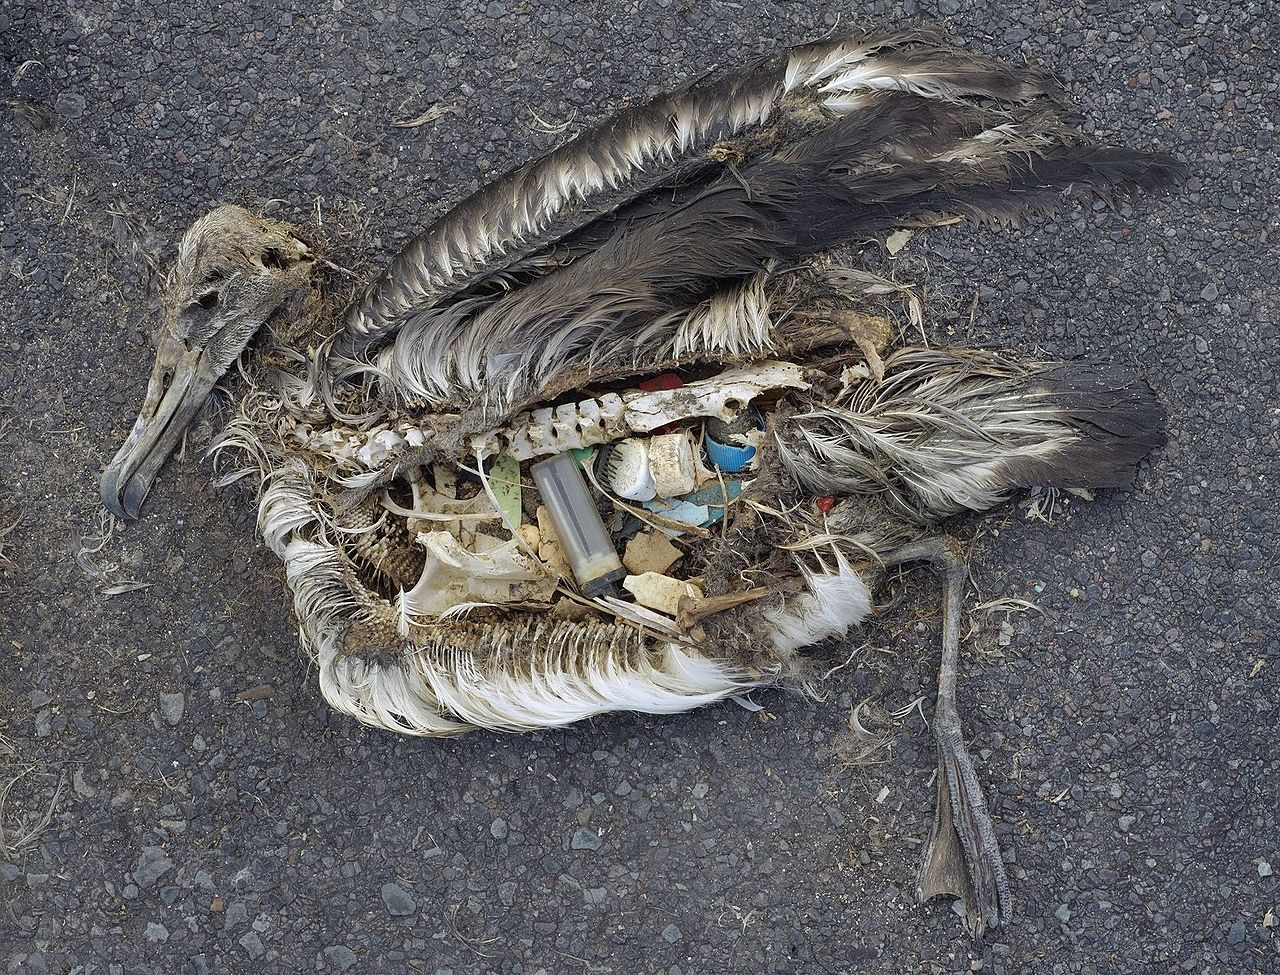
\includegraphics[height=6cm]{graphics/ChrisJordan-Albatross.jpg}
  \caption{Chris Jordan, Albatross at Midway Atoll Refuge, 2009}
  \label{fig:ChrisJordan_Albatross}
\end{figure}

The unaltered stomach contents of a dead albatross chick photographed on Midway Atoll National Wildlife Refuge in the Pacific in September 2009 include plastic marine debris fed the chick by its parents.

Using spare narration and stunning imagery, Chris Jordan's feature film MIDWAY explores the plight of Laysan albatross plagued by the ingestion of our plastic trash. Both elegy and warning, the film explores the interconnectedness of species, with the albatross on Midway as a mirror of our humanity.

Even if garbage leave outs our life, we do not care about the results of it. And it is captured by the works of Chris Jordan.In this photo series it captures 


% Effect of plastic on wildlife in Antartica.
% Her ne kadar biz çöpü attıktan bizim hayatımızdan çıksa da yok olmuyor. Sadece başka bir yerlere gidiyor. Mesela kuşların midelerine. Chris Jordan'ının imageları bunu çok da güzel açığa çıkartıyor. Bizim çöpleriminde habersiz hayvanlar bunları yiyorlar. Bir yandan ürettiğimiz ürünler ile kaynakları tüketirken bir diğer yandan ise artıklarımız diğer yaşanları tüketiyor. Dikkat çekmek istediğim nokta aslında ekolojik hassasiyetlerden çok aslında elimizde avucumuzda ne varsa onları tüketiyor olmamız. Karşı durduğum nokta ise tam olarak burası. 
